\documentclass[tikz,border=8pt]{standalone}
\usepackage{amsmath,amssymb}
\usetikzlibrary{arrows.meta,automata,positioning,quotes}
\begin{document}
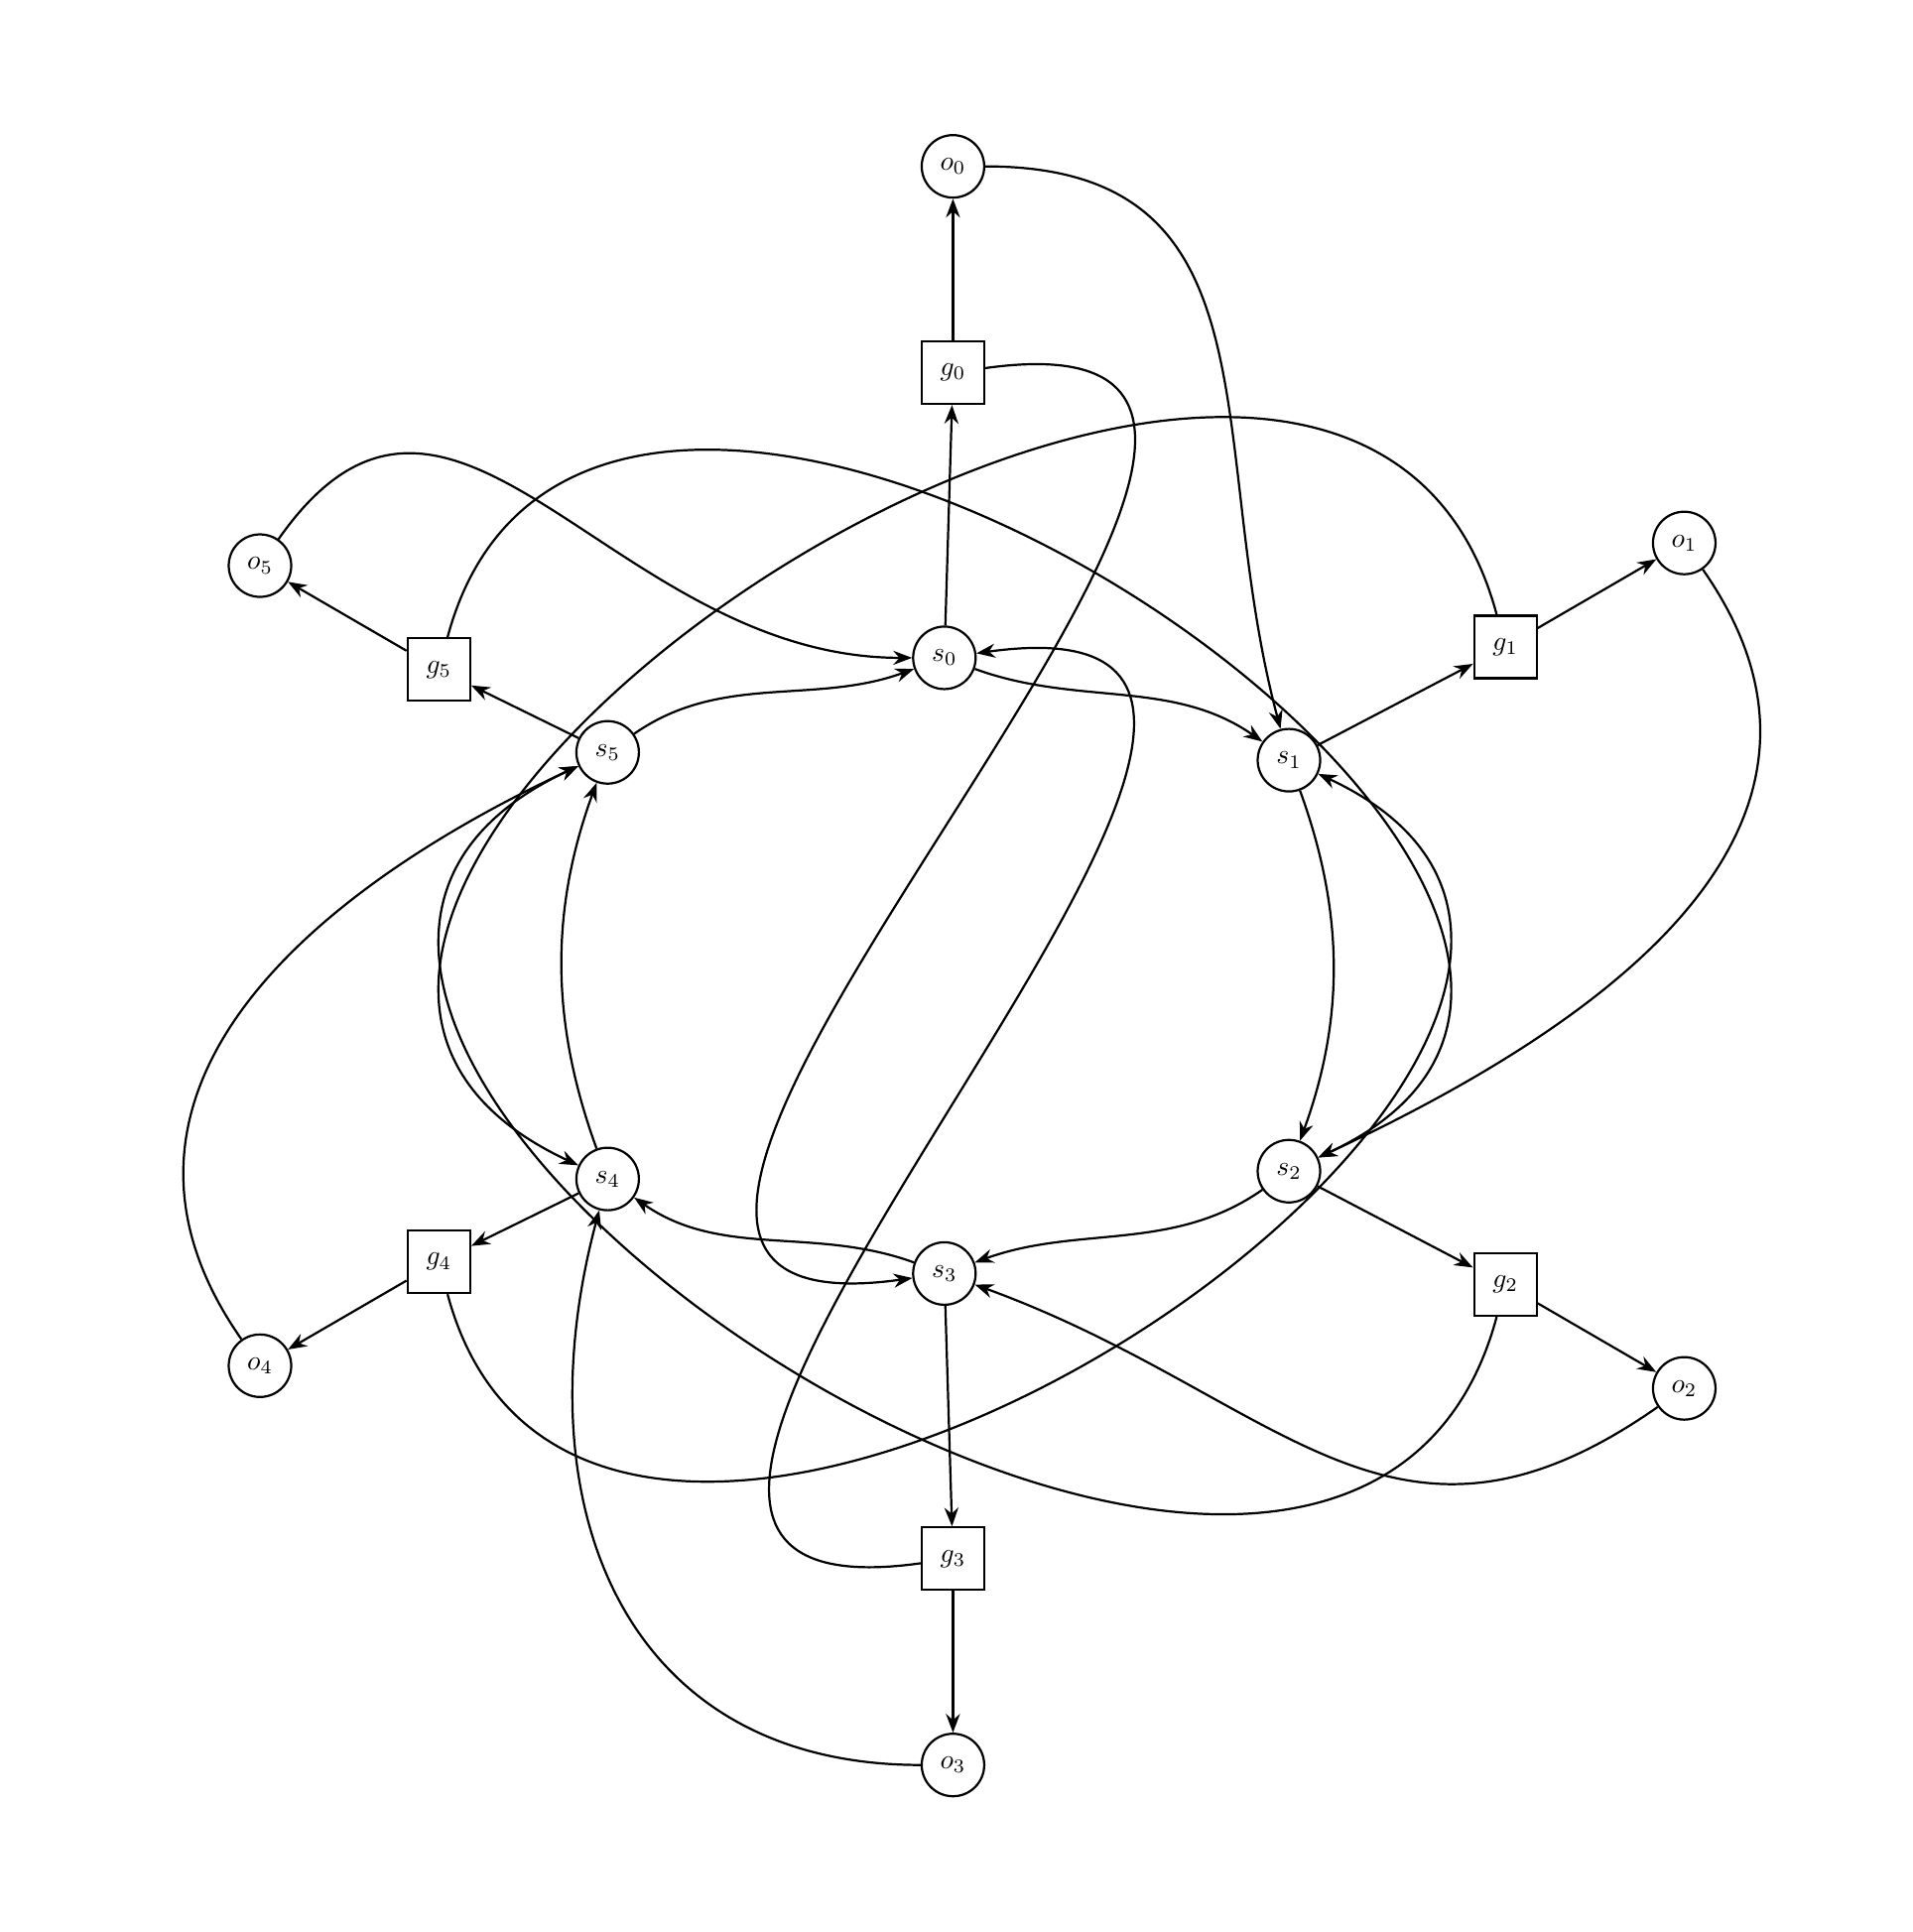
\begin{tikzpicture}[x=1cm,y=1cm]
\tikzset{
  graphnode/.style={circle,draw,thick,minimum size=8mm,inner sep=1pt,font=\sffamily},
  directed/.style={-{Stealth[length=2.4mm]},thick},
  undirected/.style={thick}
}
\node[graphnode,circle,draw] (n_s0) at (-0.12,3.94) {$s_0$};
\node[graphnode,circle,draw] (n_s1) at (4.29,2.63) {$s_1$};
\node[graphnode,circle,draw] (n_s2) at (4.29,-2.63) {$s_2$};
\node[graphnode,circle,draw] (n_s3) at (-0.12,-3.94) {$s_3$};
\node[graphnode,circle,draw] (n_s4) at (-4.43,-2.73) {$s_4$};
\node[graphnode,circle,draw] (n_s5) at (-4.43,2.73) {$s_5$};
\node[graphnode,rectangle,draw] (n_g0) at (-0.01,7.59) {$g_0$};
\node[graphnode,rectangle,draw] (n_g1) at (7.06,4.08) {$g_1$};
\node[graphnode,rectangle,draw] (n_g2) at (7.06,-4.08) {$g_2$};
\node[graphnode,rectangle,draw] (n_g3) at (-0.01,-7.59) {$g_3$};
\node[graphnode,rectangle,draw] (n_g4) at (-6.59,-3.79) {$g_4$};
\node[graphnode,rectangle,draw] (n_g5) at (-6.59,3.79) {$g_5$};
\node[graphnode,circle,draw] (n_o0) at (-0.01,10.23) {$o_0$};
\node[graphnode,circle,draw] (n_o1) at (9.35,5.41) {$o_1$};
\node[graphnode,circle,draw] (n_o2) at (9.35,-5.41) {$o_2$};
\node[graphnode,circle,draw] (n_o3) at (-0.01,-10.23) {$o_3$};
\node[graphnode,circle,draw] (n_o4) at (-8.88,-5.12) {$o_4$};
\node[graphnode,circle,draw] (n_o5) at (-8.88,5.12) {$o_5$};
\draw[directed] (n_s0) to[out=-20,in=145,looseness=0.95] (n_s1);
\draw[directed] (n_s1) to[out=-70,in=70,looseness=0.95] (n_s2);
\draw[directed] (n_s2) to[out=-145,in=20,looseness=0.95] (n_s3);
\draw[directed] (n_s3) to[out=160,in=-35,looseness=0.95] (n_s4);
\draw[directed] (n_s4) to[out=110,in=-110,looseness=0.95] (n_s5);
\draw[directed] (n_s5) to[out=35,in=200,looseness=0.95] (n_s0);
\draw[directed] (n_s0) -- (n_g0);
\draw[directed] (n_g0) -- (n_o0);
\draw[directed] (n_o0) to[out=0,in=105,looseness=1.2] (n_s1);
\draw[directed] (n_s1) -- (n_g1);
\draw[directed] (n_g1) -- (n_o1);
\draw[directed] (n_o1) to[out=-55,in=25,looseness=1.15] (n_s2);
\draw[directed] (n_s2) -- (n_g2);
\draw[directed] (n_g2) -- (n_o2);
\draw[directed] (n_o2) to[out=-145,in=-20,looseness=1.2] (n_s3);
\draw[directed] (n_s3) -- (n_g3);
\draw[directed] (n_g3) -- (n_o3);
\draw[directed] (n_o3) to[out=180,in=-105,looseness=1.2] (n_s4);
\draw[directed] (n_s4) -- (n_g4);
\draw[directed] (n_g4) -- (n_o4);
\draw[directed] (n_o4) to[out=125,in=-155,looseness=1.15] (n_s5);
\draw[directed] (n_s5) -- (n_g5);
\draw[directed] (n_g5) -- (n_o5);
\draw[directed] (n_o5) to[out=55,in=180,looseness=1.2] (n_s0);
\draw[directed] (n_g0) to[out=8,in=188,looseness=1.55] (n_s3);
\draw[directed] (n_g1) to[out=105,in=155,looseness=1.45] (n_s4);
\draw[directed] (n_g2) to[out=-105,in=-155,looseness=1.45] (n_s5);
\draw[directed] (n_g3) to[out=188,in=8,looseness=1.55] (n_s0);
\draw[directed] (n_g4) to[out=-75,in=-25,looseness=1.45] (n_s1);
\draw[directed] (n_g5) to[out=75,in=25,looseness=1.45] (n_s2);
\end{tikzpicture}
\end{document}
